%=====================================================================
%  Mini Project Report — ENGLISH version
%  Compile with: xelatex main.tex   (twice, for TOC)
%  Requires: vpcoe.cls, fancyhdr.sty, vpcoe_logo.JPG, figures/*.png
%  Devanagari support: fontspec + Nirmala UI (Windows system font).
%
%  Rebuilt from the Chinese main.tex skeleton + the translated EN PDF,
%  with three fixes applied vs the previous EN PDF (EnHi_NMT_Report.pdf):
%    1. All seven figure placeholders replaced with real graphics.
%    2. §5.1 conclusion reworded: the 1h17m figure is the final
%       verification run; the two recurrent models reused checkpoints
%       (already disclosed in §3.7).
%    3. Appendix A: "test subset 3,000" corrected to the official
%       2,505-sentence test set.
%=====================================================================
\documentclass[a4paper,12pt]{vpcoe}
\usepackage{graphicx}
\usepackage{fancyhdr}
\usepackage{booktabs}
\usepackage{amsmath}
\usepackage{float}
% The class sets \textwidth manually and ignores the a4paper option, so the page
% would otherwise come out US Letter. Force A4 with symmetric margins.
\usepackage[a4paper,left=3.0cm,right=2.5cm,top=2.5cm,bottom=2.5cm,includefoot]{geometry}
% Devanagari for the original Hindi model output (Windows system font).
\usepackage{fontspec}
\newfontfamily\devfont[Script=Devanagari]{Nirmala UI}
% vpcoe.cls declares \newif\iftablespage and \newif\iffigurespage, both defaulting
% to FALSE, so \makecontents silently emits only the table of contents. These must
% be set in the PREAMBLE, before \makecontents is called.
\tablespagetrue
\figurespagetrue

\pagestyle{bfheadings}
\pagestyle{fancy}
% --- visual-judge fixes: header collision + near-empty float pages ---
% Wrap both running heads in parboxes so long section titles wrap instead of
% overlapping the chapter mark on the same line.
\fancyhead[L]{\parbox[t]{0.60\textwidth}{\footnotesize\itshape\nouppercase{\leftmark}}}
\fancyhead[R]{\parbox[t]{0.34\textwidth}{\raggedleft\footnotesize\itshape\nouppercase{\rightmark}}}
% Stop LaTeX from creating float pages that are almost empty.
\renewcommand{\floatpagefraction}{.85}
\renewcommand{\textfraction}{.1}
\renewcommand{\topfraction}{.9}
\renewcommand{\bottomfraction}{.9}

\begin{document}

\begin{frontmatter}

%--------------------------------------------------------------- title page
\begin{dedication}
\begin{center}

\includegraphics[width=3cm, height=3cm]{vpcoe_logo.JPG}\\
\Large{Mini Project Report on} \\
\Titlefnt{English $\rightarrow$ Hindi Neural Machine Translation: A Comparative Study of Three Sequence-to-Sequence Architectures}\\
\vskip 0.30in
\Large{Submitted in fulfillment of activity requirements} \degfntbf{in the subject Deep Learning} \\
\vskip 0.05in
\textsc{by} \\
\textbf{Anish Charudatta Date} \\
\textbf{Roll No. EN25552003}\\
\vskip 0.2in
\Large{Under the guidance of} \\
\Large{Prof. Sushma S. Nandgaonkar} \\
\vskip 0.4in
\Large{Vidya Pratishthan's}\\
\Large{Kamalnayan Bajaj Institute of Engineering and Technology} \\
\Large{Baramati-413133, Dist-Pune (M.S.) India}\\
\Large{Department of Computer Engineering} \\
\Large{November 2026-27}
\end{center}
\end{dedication}

%--------------------------------------------------------------- certificate
\begin{dedication}
\begin{center}

\includegraphics[width=3cm, height=3cm]{vpcoe_logo.JPG}\\
\Large{VPKBIET, Baramati} \\
\vskip 0.3in
\Certfnt{Certificate} \\
\large{This is to certify that the Mini Project Report on} \\
\Titlefnt{English $\rightarrow$ Hindi Neural Machine Translation: A Comparative Study of Three Sequence-to-Sequence Architectures} \\
\vskip 0.2in
\textsc{submitted by} \\
\textbf{Anish Charudatta Date} \\
\textbf{Roll No. EN25552003}\\
\large{in fulfillment of the activity requirements in the subject Deep Learning at Vidya Pratishthan's Kamalnayan Bajaj Institute of Engineering and Technology, Baramati, under the Savitribai Phule Pune University, Pune. This work is done during year 2026-27 Semester-III, under our guidance.} \\
\vskip 0.75in
\large{Prof. Sushma S. Nandgaonkar} \hspace{1.2cm}
\large{Dr. A.M.Jagtap} \hspace{1.2cm}
\large{Dr. S.B.Lande } \\
\hspace{-1cm}
\large{Mini Project Guide} \hspace{70pt}
\large{Head of Dept.} \hspace{80pt}
\large{Principal}\\
\end{center}
\vskip 0.50in
\large{Examiner 1:-------} \hspace {7cm} \large{Examiner 2: - - - - - - -}
\end{dedication}

\end{frontmatter}

%--------------------------------------------------------------- front matter
\acknowledgements
I would like to express my sincere gratitude to my mini project guide, Prof.~Sushma S. Nandgaonkar, for her continuous guidance, patient review and constructive criticism throughout this work. I am grateful to the Department of Computer Engineering for providing the computational facilities that made the experiments possible. I also thank Dr.~A.~M.~Jagtap, Head of the Department of Computer Engineering, Dr.~S.~B.~Lande, Principal of VPKBIET, and all the faculty members of the department, for their support and encouragement. I thank IIT Bombay for making the English--Hindi parallel corpus publicly available, and the Hugging Face and SentencePiece communities, without whose open-source tools this study could not have been reproduced. I also thank my classmates for their comments during the preparation of this report.

\begin{abstract}
English to Hindi is a comparatively under-resourced translation pair, and Hindi is morphologically rich, so a word-level vocabulary degenerates into \texttt{<unk>} for a large fraction of tokens. This makes the architecture comparisons reported in the literature hard to trust: most of them change the tokeniser, the data budget and the training schedule at the same time as the model, so the contribution of the architecture itself is confounded.

This report presents a controlled comparison of three sequence-to-sequence architectures under a fixed budget: a vanilla LSTM encoder--decoder, a Seq2Seq model with Bahdanau additive attention, and a Transformer. All three share one data-cleaning pipeline, one SentencePiece subword tokeniser, one training loop and one decoding routine; the only variable is the model itself.

The data is the IIT Bombay English--Hindi parallel corpus. The raw training split contains 1,652,981 pairs, of which 83.3\% survive cleaning. A budgeted subset of 99,561 pairs is used for training, with 3,000 pairs for validation and 2,505 for testing. Tokenisation uses SentencePiece Unigram models with 32,000 subword units per language.

The tokenisation result is the most striking single finding. The word-level vocabulary produces a Hindi \texttt{<unk>} rate of 8.85\% on the test set; subword tokenisation reduces it to 0.001\%, a difference of roughly four orders of magnitude.

On the model comparison, the Bahdanau attention model performs best, reaching chrF++ 18.56 and BLEU 2.665 under greedy decoding; the vanilla LSTM reaches 14.80 and 1.334; the Transformer reaches 7.91 and 0.427. Architecture therefore buys a spread of 10.65 chrF++ points at this budget.

The training instability of the Transformer is treated in a section of its own. With the original Noam learning rate (peak $6.99\times10^{-4}$) the model diverged at epoch 5 and degenerated into repetitive output. Reducing the peak to $3.84\times10^{-4}$ restored stable training and raised chrF++ from 3.49 to 7.91. We attribute the divergence to the fact that a batch here contains about 4,000 tokens, far below the roughly 25,000 that the Noam schedule assumes.

The conclusion is that at a hundred-thousand-pair budget the benefit of attention is clear and measurable, while the Transformer remains limited by data scale and does not yet show its advantage.
\end{abstract}

\makecontents
% NOTE: \makecontents (defined in vpcoe.cls) already emits \tableofcontents,
% \listoftables and \listoffigures. Do NOT add them again here — a second
% \listoffigures reads an already-truncated .lof and prints an empty page.

\keywords
{\large\bf{Keywords---}}
Neural Machine Translation; English--Hindi; Sequence-to-Sequence; Bahdanau Attention; Transformer; SentencePiece; BLEU; chrF++; TER

\vspace{10MM}
\noindent
\large{Abbreviations---} NMT, RNN, LSTM, GRU, BLEU, chrF++, TER, OOV, SP, AMP, GPU, T4.

\notations
\large{Notation is limited to standard NMT symbols: $\mathbf{x}_{1..m}$ for source tokens, $\mathbf{y}_{1..n}$ for target tokens, $\theta$ for model parameters, and $\alpha$ for the length-normalisation factor.}

\renewcommand{\footrulewidth}{1pt}
\lfoot{English $\rightarrow$ Hindi NMT: A Comparative Study \\ of Three Sequence-to-Sequence Architectures}
\rfoot{VPKBIET, Baramati}

%=====================================================================
\chapter{Introduction}

\section{Research Background}
English-to-Hindi is one of the most important machine-translation directions on the Indian subcontinent, yet the scale of its parallel corpora is far smaller than that of traditional pairs such as English--German or English--French. Taking the public IIT Bombay corpus as an example, the usable training pairs number about 1.6 million, an order of magnitude below the tens of millions of pairs at WMT scale. Under such data conditions, the trade-off between model choice and training strategy is more sensitive than in high-resource settings.

Over the past decade and more, the technical route of this direction has undergone a whole-scale migration from statistical machine translation (SMT) to neural machine translation (NMT). The sequence-to-sequence framework proposed by Sutskever et al.\ encodes and decodes with two recurrent neural networks, making end-to-end training possible for the first time; Bahdanau et al.\ then introduced additive attention, relieving the information bottleneck of the fixed-length context vector; and the Transformer proposed by Vaswani et al.\ replaced recurrent structure entirely with self-attention, achieving marked advantages on high-resource language pairs.

For a practitioner, deploying a translation system requires three decisions at once: which architecture to adopt, whether to use word-level or subword-level tokenisation, and how much data and compute to invest. The three interact, and most comparative conclusions in the existing literature were obtained under high-resource, multi-GPU, long-schedule conditions; transferring them directly to a single-GPU, hundred-thousand-pair setting need not hold.

\begin{figure}[htbp]
\centering
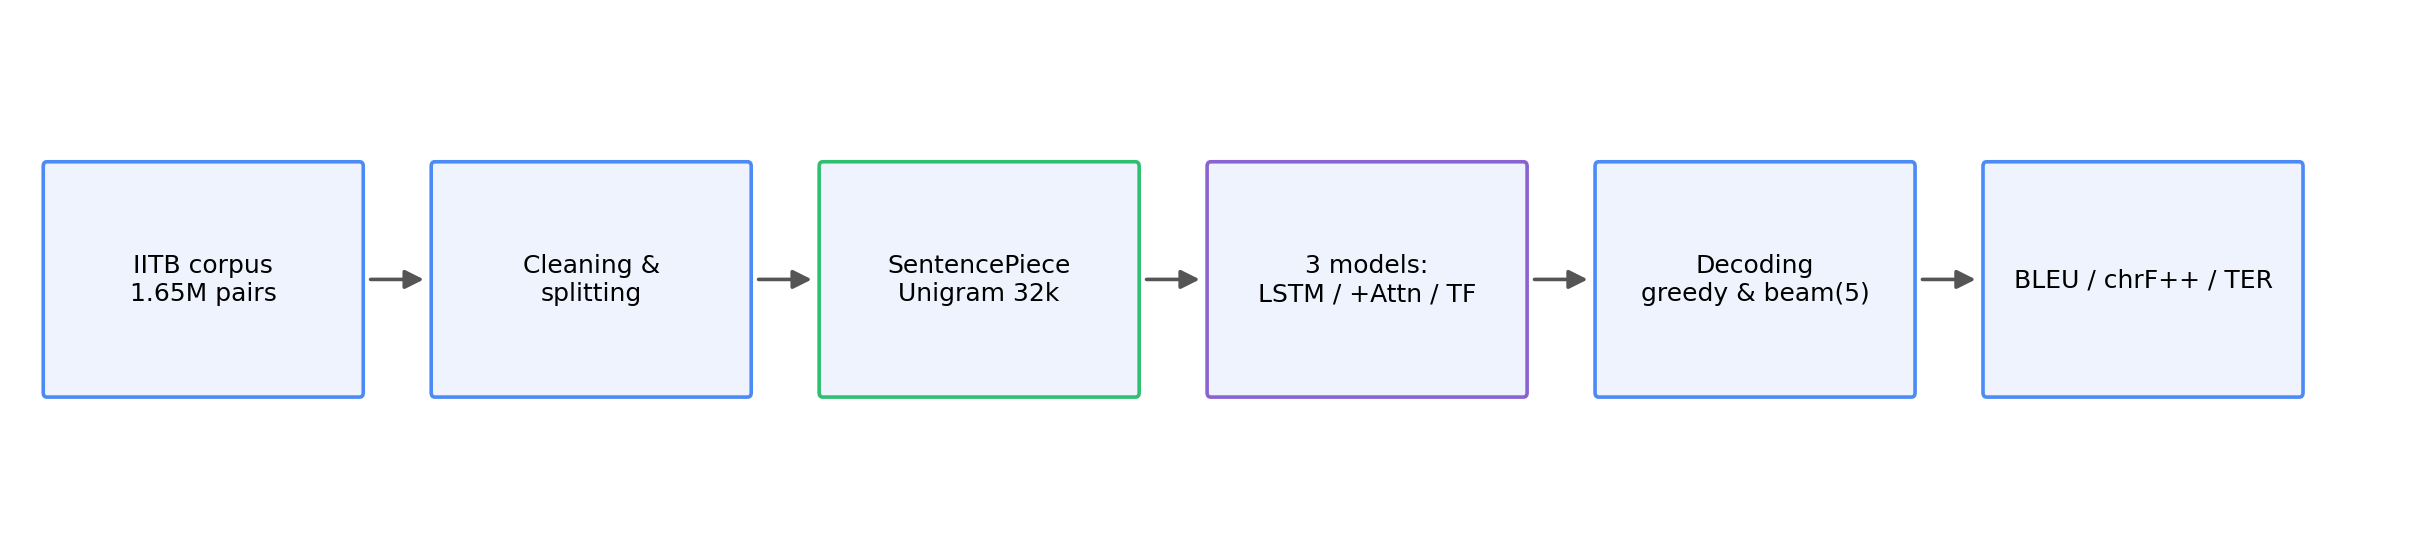
\includegraphics[width=0.98\textwidth]{figures/00_pipeline_schematic.png}
\caption{The experimental pipeline shared by the three architectures.}
\label{fig:pipeline}
\end{figure}

\section{Problem Statement}
The core question of this study is: under a fixed data and compute budget, how much performance difference does the architecture itself buy?

This question is worth studying on its own for two reasons.

First, Hindi is a morphologically rich language: nouns inflect for gender, number, and case, and verbs combine person, tense, and aspect. A word-level vocabulary covers only high-frequency word forms on the training set; at test time a large number of low-frequency forms degenerate to \texttt{<unk>}. The measurements of this study show that, under a word-level vocabulary, the out-of-vocabulary rate on the Hindi test set is 8.85\%, meaning nearly one token in ten loses its semantics at inference.

Second, if the tokenisation is changed at the same time as the architecture, the effects of the two variables entangle. For instance, if one architecture performs better, that may be because it suits subword representations better, or simply because subword splitting itself reduced the OOV count. Unless tokenisation is fixed as a constant, the contribution of architecture cannot be identified separately.

This study therefore fixes the tokenisation, data scale, batch size, number of training epochs, and evaluation metrics, and varies only the model structure, in order to obtain an interpretable comparison.

\section{Motivation}
Published architecture-comparison studies usually vary several factors at once: different data scales, different tokenisers, different use of pretrained weights, different training durations. Such studies are meaningful for ``which option is strongest in absolute performance,'' but cannot answer ``under equal investment, is switching architecture worth it.''

For resource-limited researchers and engineering teams, the latter question is usually the more practical one. A model trained on eight GPUs for two weeks and a model trained on one GPU for one hour do not constitute directly transferable advice, even if the former scores higher.

This study therefore presses the budget down to a concrete and reproducible level: a single Kaggle T4$\times$2 session, a training subset of one hundred thousand pairs, a twelve-epoch cap, and no pretrained weights of any kind. The architecture ranking obtained under this budget is a useful reference for users under comparable resource conditions.

\section{Main Contributions}
The work of this report can be summarised in three points.
\begin{itemize}
  \item A complete pipeline shared by all three architectures. Data cleaning, subword splitting, batch construction, the training loop, checkpoint management, decoding, and metric computation all share one and the same implementation; the three models differ only in their structure definitions, so the comparison is not contaminated by implementation differences.
  \item The tokenisation effect is measured rather than assumed. We tabulate separately the test-set out-of-vocabulary rates of the word-level and subword vocabularies, obtaining 8.85\% and 0.001\%, and take these two numbers as the premise of all subsequent discussion.
  \item BLEU, chrF++, and TER are reported under both greedy and beam-search decoding. A single metric misleads easily, especially on a morphologically rich target language such as Hindi, where a translation with low word-level overlap can be semantically perfect; chrF++ is therefore the primary ranking criterion and BLEU the auxiliary.
\end{itemize}

\section{Organisation of the Report}
Chapter 2 states the research objectives and scope; Chapter 3 details the data, tokenisation, models, training, and evaluation methods; Chapter 4 presents the experimental results and develops the discussion; Chapter 5 summarises the conclusions, limitations, and future work.

%=====================================================================
\chapter{Research Objectives and Scope}

\section{Research Objectives}
This study sets five objectives.
\begin{enumerate}
  \item Build a reproducible English-to-Hindi pipeline on the IIT Bombay English--Hindi parallel corpus, covering the full flow of cleaning, splitting, subword tokenisation, training, decoding, and evaluation.
  \item Quantitatively measure the difference in out-of-vocabulary rates between the word-level and subword vocabularies on the same test set, demonstrating the necessity of subword splitting with numbers.
  \item Train three architectures under an exactly identical training recipe: a vanilla LSTM encoder--decoder, a Seq2Seq with Bahdanau additive attention, and a Transformer.
  \item Compare the three architectures under greedy decoding and beam search using BLEU, chrF++, and TER.
  \item Analyse the failure modes of each model, including performance bucketed by source-sentence length, attention-alignment patterns, and typical error types.
\end{enumerate}

\section{Research Scope}
Within the scope of this study are: one-way English-to-Hindi translation; the IIT Bombay corpus; a training subset of one hundred thousand pairs; SentencePiece Unigram subword models with 32,000 units per language; a single seed (seed 42); and all models trained from scratch without pretrained weights.

Outside the scope of this study are: multilingual joint training; pivot translation between low-resource languages; domain adaptation; model compression and deployment optimisation; and interactive or online learning.

\section{Constraints}
The experiments are completed within a single Kaggle Notebook session on two NVIDIA Tesla T4 GPUs with 15.6~GB of memory each. Under the memory limit, the batch size is fixed at 128 sentences with a maximum subword length of 128; under the session-duration limit, the epoch cap is set to 12 with early stopping. All experiments use a fixed random seed with no multi-seed repetition; this report therefore gives no error bars.

\begin{table}[h]
\centering
\caption{Research objectives and their verification methods.}
\label{tab:objmap}
\begin{tabular}{@{}lll@{}}
\toprule
Objective & Verification & Reported in \\
\midrule
O1 Pipeline & End-to-end run with artifacts written to disk & \S 3.7 \\
O2 Tokenisation & Word-level OOV \% vs.\ subword \texttt{<unk>} \% & Table 4.1 \\
O3 Training & Best epoch, validation loss & Table 4.2 \\
O4 Comparison & BLEU / chrF++ / TER, greedy and beam & Table 4.3 \\
O5 Analysis & Length-bucketed chrF++, heatmap, error samples & \S 4.5--4.7 \\
\bottomrule
\end{tabular}
\end{table}

%=====================================================================
\chapter{Methodology}

\section{Dataset}
The experiments use the IIT Bombay English--Hindi parallel corpus \cite{kunchukuttan2018}, one of the most widely used public benchmarks for this language pair. The raw split contains 1,652,981 training pairs, 520 validation pairs, and 2,507 test pairs.

The sentence-length distribution (in words) shows a pronounced long tail: English averages 13.1 words, median 9, 90th percentile 30, 99th percentile 68, maximum 1,917; Hindi averages 14.1 words, median 9, 90th percentile 33, 99th percentile 76, maximum 1,380. Hindi runs about one word longer than English on average, consistent with the morphological difference between the two languages---Hindi postpositions and inflectional endings often correspond to English prepositions and auxiliaries.

There are four cleaning rules: unified Unicode normalisation (NFKC on the source side, NFC on the target side); removal of exact-duplicate sentence pairs; verification that the target side contains Devanagari characters, dropping samples mixed with other scripts or empty strings; and filtering by source/target length ratio, dropping anomalous pairs whose ratio exceeds 3.0. The final truncation acts on subword sequences, with a threshold of 128 subword units.

\begin{table}[h]
\centering
\caption{Corpus splits after cleaning and subsampling.}
\label{tab:splits}
\begin{tabular}{@{}lrrr@{}}
\toprule
Split & Raw pairs & After cleaning & Used in this study \\
\midrule
Training   & 1,652,981 & 1,377,338 & 99,561 \\
Validation &       520 &       520 &  3,000 \\
Test       &     2,507 &     2,505 &  2,505 \\
\bottomrule
\end{tabular}

\vspace{2pt}
{\footnotesize The training set retains 83.3\% after deduplication and length-ratio filtering. The 99,561 is the 100,000 pairs drawn from the official training set minus 439 pairs dropped for exceeding the length limit after subword encoding. The validation set is the official 520 pairs plus 2,480 pairs carved from the official training set outside the 100,000-pair subset, so the 99,561-pair training subset is unaffected; the official test set contains 2,505 pairs after cleaning.}
\end{table}

\begin{figure}[h]
\centering
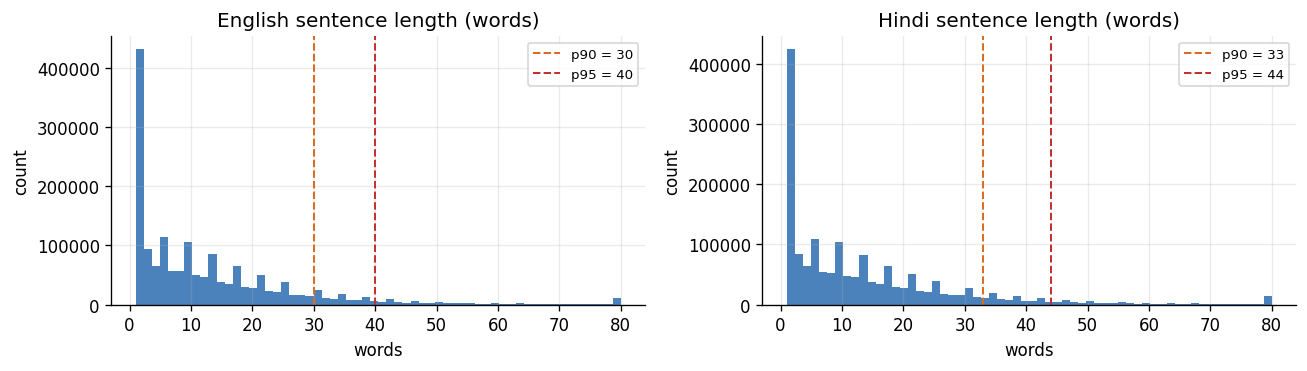
\includegraphics[width=0.98\textwidth]{figures/01_length_distribution.png}
\caption{Sentence-length distribution before filtering.}
\label{fig:lengthdist}
\end{figure}

\section{Tokenisation}
Word-level baseline: a word-level vocabulary is built on the hundred-thousand training pairs (minimum frequency 2); the English vocabulary is 49,955 with a test-set OOV rate of 11.97\%; the Hindi vocabulary is 43,774 with an OOV rate of 8.85\%. Although the Hindi OOV rate is lower than the English one, the absolute value remains high. The reason is that Hindi inflection is far richer than English's: a single root can derive dozens of inflected forms, each form's frequency is diluted, and few cross the minimum-frequency threshold.

Subword model: switching to SentencePiece (Unigram algorithm) \cite{kudo2018}, the vocabulary per language is fixed at 32,000 subword units, with special symbols numbered pad=0, unk=1, bos=2, eos=3, and byte fallback disabled. The Unigram model learns segmentation by iteratively pruning the vocabulary and re-estimating the language model, which segments morphologically rich languages fairly naturally.

How the OOV rate is measured: the same test sentences are encoded with the word-level vocabulary and with the subword model separately, and the proportion of \texttt{<unk>} tokens over all tokens is tabulated. The results appear in Section 4.1---8.85\% word-level versus 0.001\% subword, a gap of roughly four orders of magnitude. This result constitutes the premise of all subsequent comparisons: only under subword representations do the three architectures face the same, almost OOV-free input space, and only then can architectural differences be compared cleanly.

\section{Model Architectures}
The three models implement a unified abstract interface: \texttt{encode} returns the encoder memory, masks, and the decoder's initial state; \texttt{decode\_step} returns the logits of the current step and the updated state. During training a unified forward process unrolls over time steps; at inference, greedy or beam search calls the same step interface. This design guarantees that the three models share exactly the same training and decoding code, with differences confined to the internals of the two interfaces.

\subsection{Vanilla LSTM Encoder--Decoder}
Single-vector bottleneck: the encoder is a single-layer bidirectional LSTM with word-embedding dimension 300 and hidden dimension 512; the bidirectional concatenation yields an output dimension of 1,024, and input sequences are packed in descending length to skip padding positions. The decoder is initialised with the encoder's final state; at each step it takes the previous target-word embedding as input, and its output is mapped onto the target vocabulary by a linear layer \cite{sutskever2014,cho2014}. This model contains no attention: all encoder information must be compressed into one fixed-dimensional vector, making it the fixed-vector baseline of this study.

\subsection{Seq2Seq with Bahdanau Attention}
Building on the previous section, the encoder output is no longer compressed into a single vector; all time-step hidden states are kept as a memory matrix. At each decoding step the current decoder hidden state serves as the query; additive attention scores are computed against the memory matrix, normalised by softmax, and weighted-summed into a context vector, which is concatenated with the current word embedding and fed to the decoder \cite{bahdanau2015}. The attention dimension is set to 512. The output layer takes the concatenation of the decoder hidden state, the context vector, and the word embedding, so that the model can directly access different source positions when generating each word.

\subsection{Transformer}
A standard encoder--decoder structure is used: four encoder and four decoder layers, each containing multi-head self-attention and a feed-forward network; 8 heads, model dimension 512, feed-forward dimension 2,048; positional information is injected by sinusoidal position encodings \cite{vaswani2017}. Sub-layers use post-layer-normalisation with residual connections; decoder self-attention uses an upper-triangular causal mask, and cross-attention takes the encoder output as keys and values. The target word embeddings and the output projection share weights, saving about 16 million parameters and acting as regularisation. Training uses label smoothing 0.1 and the Noam learning-rate schedule with 4,000 linear warmup steps.

\begin{figure}[h]
\centering
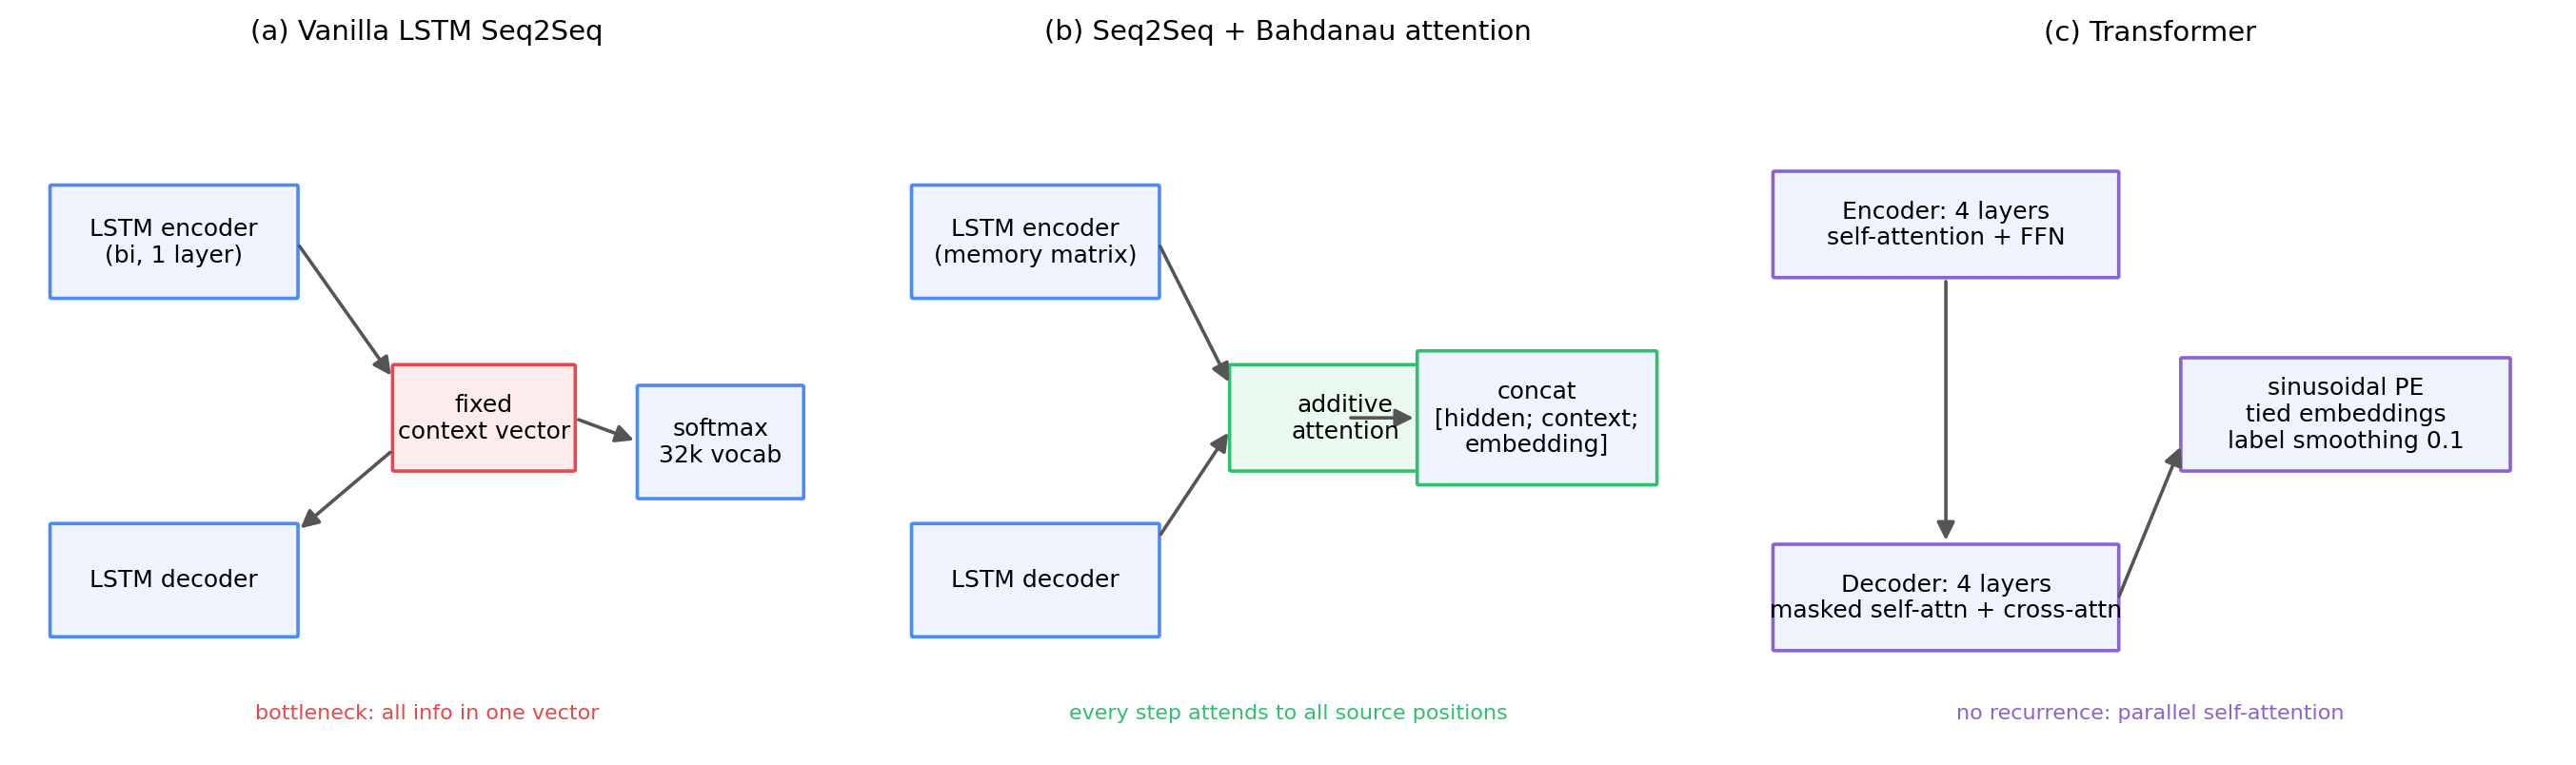
\includegraphics[width=0.98\textwidth]{figures/00_architectures.png}
\caption{Comparison of the three architectures.}
\label{fig:archs}
\end{figure}

\begin{table}[h]
\centering
\caption{Model configurations and parameter counts.}
\label{tab:models}
\begin{tabular}{@{}lrrr@{}}
\toprule
 & Vanilla LSTM & + Bahdanau & Transformer \\
\midrule
Embedding / $d_{model}$ & 300 & 300 & 512 \\
Hidden dim / layers & 512 / 1 & 512 / 1 (bidirectional) & 4+4 layers, 8 heads \\
FFN / attention dim & --- & 512 & 2,048 \\
Dropout & 0.3 & 0.3 & 0.1 \\
Parameters & 43.15 M & 94.80 M & 62.23 M \\
\bottomrule
\end{tabular}

\vspace{2pt}
{\footnotesize Introducing attention more than doubles the parameter count (43.15 M $\rightarrow$ 94.80 M), while the Transformer sits between the two in parameters.}
\end{table}

\section{Training Protocol}
The three models share one training loop and differ only in hyperparameters set according to architectural characteristics. Shared part: the optimiser is Adam ($\beta_1=0.9$, $\beta_2=0.98$, $\varepsilon=10^{-9}$); gradient clipping at 1.0; mixed-precision training enabled; batch size 128 sentences with maximum subword length 128; random seed fixed at 42; after each epoch a checkpoint is saved and the training loss, validation loss, learning rate, and wall time are recorded; early stopping is based on validation loss with the best checkpoint restored.

The per-model parts are given in the table below. The two recurrent models use plateau decay: if the validation loss does not decrease for one epoch the learning rate is halved, down to a floor of $10^{-5}$. The Transformer uses the Noam schedule, in which the learning rate rises linearly with the step count and then decays with the inverse square root of the step count.

\begin{table}[h]
\centering
\caption{Training hyperparameters per model.}
\label{tab:hparams}
\begin{tabular}{@{}lrrr@{}}
\toprule
 & Vanilla LSTM & + Bahdanau & Transformer \\
\midrule
LR schedule & ReduceLROnPlateau & ReduceLROnPlateau & Noam \\
Learning rate & $1\times10^{-3}$ & $1\times10^{-3}$ & 0.55 (peak $3.84\times10^{-4}$) \\
Warmup steps & --- & --- & 4,000 \\
Label smoothing & 0.0 & 0.0 & 0.1 \\
Early-stopping patience & 3 & 3 & 4 \\
\bottomrule
\end{tabular}

\vspace{2pt}
{\footnotesize The Transformer's learning-rate scale factor is 0.55 rather than the default 1.0; the reason is given in \S 4.8. In brief, the default Noam peak is designed for batches of about 25,000 tokens, whereas the batches here contain only about 4,000 tokens, so gradient noise is markedly larger and the default peak causes training to diverge.}
\end{table}

\section{Decoding}
Greedy decoding: at each step the argmax of the logits is emitted; decoding stops at the end symbol, with a maximum length of 128 steps.

Beam search: beam width $k=5$, length-penalty exponent $\alpha=0.7$; candidate sequences are ranked by length-normalised cumulative log-probability.

The two decodings differ in evaluation-set size: greedy decoding is evaluated on all 2,505 test sentences, whereas beam search is evaluated on the first 1,000 only. This is a compromise between compute cost and statistical reliability---beam search costs about 5 to 20 times greedy per sentence, and running it on the full set would consume too much of the session time.

\section{Evaluation Metrics}
Three automatic metrics are used, all computed with sacrebleu.

BLEU: based on word-level n-gram precisions ($n=1\ldots4$) with a brevity penalty, using the \texttt{intl} tokenizer to suit multilingual settings \cite{papineni2002}. Its limitation is that it counts surface-form overlap only and is insensitive to paraphrase and word-order changes.

chrF++: an F-score over character-level n-grams augmented with a word-level bigram term \cite{popovic2017}. For a morphologically rich target language such as Hindi, where one meaning can be expressed by many word forms, character-level metrics are far more forgiving than word-level ones; this study therefore uses chrF++ as the primary ranking criterion.

TER: translation edit rate, the ratio of the minimum number of edit operations needed to turn the hypothesis into the reference to the reference length \cite{snover2006}. Lower is better, opposite in direction to BLEU and chrF++.

A caveat must be stated: on the 2,505-sentence test set the confidence interval of BLEU is about $\pm0.5$ to $\pm1.0$. This report therefore does not treat BLEU differences within 0.3 points as valid differences; ranking is by chrF++ throughout.

\section{Implementation Environment}
The experiments run on PyTorch 2.x and CUDA \cite{paszke2019}, in Kaggle Notebooks batch mode, on two NVIDIA Tesla T4 GPUs (15.6 GB each). Tokenisation uses SentencePiece and evaluation uses sacrebleu. All experiments fix the random seed and enable benchmark mode for CUDA convolution algorithms to improve throughput. One complete run (data preparation, training, and evaluation) takes 1 hour 17 minutes of wall time; across the two GPUs this corresponds to about 2.6 GPU-hours (weekly quota 30 hours).

Training supports checkpoint resumption: if a model file exists and its history shows that training completed or early-stopped, training of that model is skipped and the weights are loaded directly. This mechanism saved substantial compute during the iteration of this study---when the Transformer learning rate was fixed and runs repeated, the two recurrent models were reused directly and only the Transformer was retrained.

%=====================================================================
\chapter{Results and Discussion}

\section{Tokenisation Effect}
The most definitive single result of this study is the effect of tokenisation on the out-of-vocabulary rate.

\begin{table}[h]
\centering
\caption{Out-of-vocabulary rates on the test set.}
\label{tab:unk}
\begin{tabular}{@{}lrr@{}}
\toprule
Tokenisation & Hindi vocabulary size & Token-level \texttt{<unk>} rate \\
\midrule
Word-level (min.\ frequency 2) & 43,774 & 8.85\,\% \\
SentencePiece Unigram & 32,000 & 0.001\,\% \\
\bottomrule
\end{tabular}

\vspace{2pt}
{\footnotesize Measured on the 2,505-sentence test set. Under subword splitting the proportion of sentences containing \texttt{<unk>} is 0.0\%. On the English side the rate falls from 11.97\% word-level to 0.000\%.}
\end{table}

Under the word-level vocabulary, nearly one test token in ten cannot be represented; with subwords, that proportion falls to the parts-per-million level. This gap is about four orders of magnitude.

The significance of this result lies beyond the numbers themselves. It shows that under a word-level setup the performance ceiling of any architecture is heavily suppressed by OOVs; comparing architectures in that regime measures mostly ``which model guesses OOVs better from context'' rather than the modelling capacity of the architecture itself. Only under subword representations do the three architectures face the same, almost unknown-free input space, and only then is an architectural comparison meaningful. All subsequent experiments of this study are therefore conducted in the subword setting.

\section{Training Behaviour}
The three models differ markedly in their convergence behaviour.

\begin{table}[h]
\centering
\caption{Training results and wall time of the three models.}
\label{tab:training}
\begin{tabular}{@{}lrrrrrr@{}}
\toprule
Model & Params & Best epoch & Best val.\ loss & Perplexity & Final train loss & Train time \\
\midrule
Vanilla LSTM & 43.15 M & 10 & 4.6957 & 109.48 & 3.6672 & 51.2 min \\
+ Bahdanau & 94.80 M & 6 & 4.3803 & 79.86 & 2.6522 & 120.8 min \\
Transformer & 62.23 M & 7 & 6.5154 & 675.49 & 6.7155 & 59.0 min \\
\bottomrule
\end{tabular}
\end{table}

In convergence speed, the Bahdanau model reaches its best validation loss 4.3803 at epoch 6, the lowest of the three; the vanilla LSTM reaches 4.6957 at epoch 10; the Transformer reaches 6.5154 at epoch 7, with perplexity as high as 675, far above the two recurrent models.

In wall time, Bahdanau takes about 13.4 minutes per epoch, the vanilla LSTM about 4.3 minutes, and the Transformer about 5.1 minutes. Bahdanau is the slowest because its decoder unrolls serially over time steps and it has the largest parameter count.

As signs of overfitting: the vanilla LSTM's validation loss begins to rise after epoch 10 (4.7056 at epoch 11, 4.7117 at epoch 12) while its training loss keeps falling to 3.6672---mild overfitting; the 12-epoch cap ended training and the best (epoch-10) checkpoint was restored. Bahdanau's validation loss fails to decrease for three consecutive epochs after epoch 6 and early-stops at epoch 9. The Transformer shows clear oscillation after epoch 7; see \S 4.8.

\begin{figure}[h]
\centering
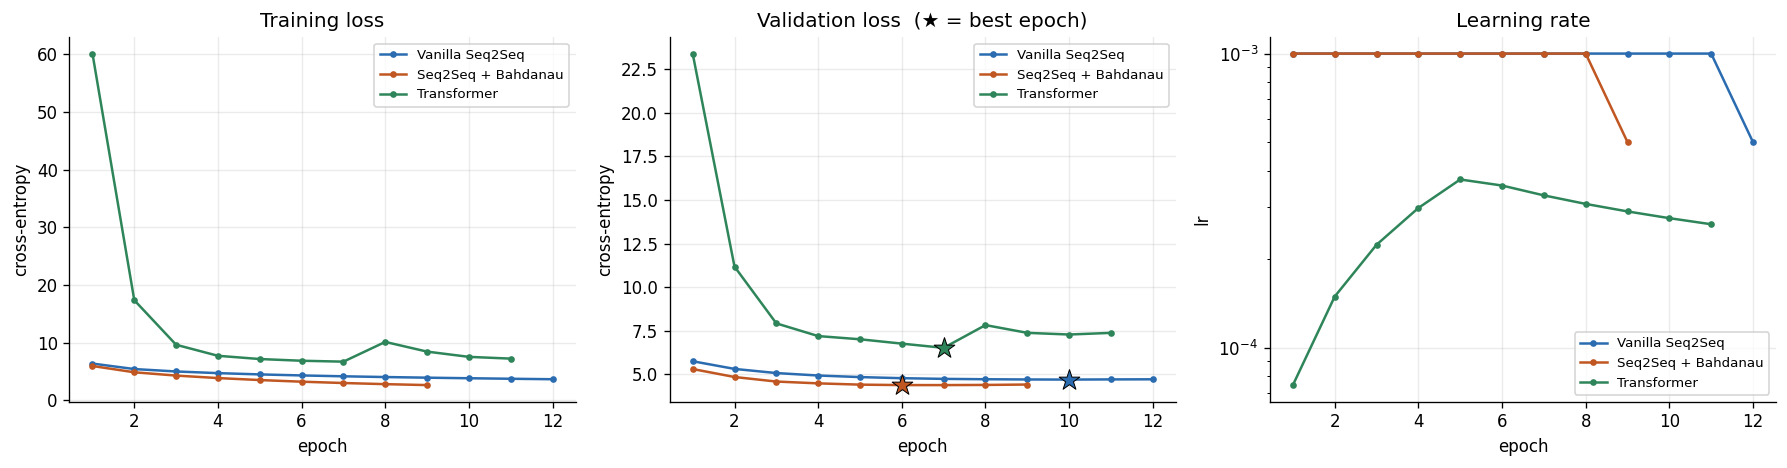
\includegraphics[width=0.98\textwidth]{figures/02_training_curves.png}
\caption{Training and validation loss curves of the three models; stars mark the best epoch.}
\label{fig:curves}
\end{figure}

\section{Main Comparison Results}
The complete results of the three models on the test set are as follows (greedy decoding $n=2{,}505$, beam search $k=5$, $n=1{,}000$).

\begin{table}[h]
\centering
\caption{Main results on the test set (corpus-level).}
\label{tab:main}
\begin{tabular}{@{}lrrrrrr@{}}
\toprule
 & \multicolumn{3}{c}{Greedy decoding} & \multicolumn{3}{c}{Beam search ($k=5$)} \\
\cmidrule(lr){2-4}\cmidrule(lr){5-7}
Model & BLEU & chrF++ & TER & BLEU & chrF++ & TER \\
\midrule
Vanilla LSTM & 1.334 & 14.796 & 100.814 & 1.524 & 13.649 & --- \\
+ Bahdanau   & \textbf{2.665} & \textbf{18.560} & \textbf{98.656} & \textbf{3.307} & \textbf{17.929} & --- \\
Transformer & 0.427 & 7.911 & 213.607 & 0.941 & 9.094 & --- \\
\bottomrule
\end{tabular}
\end{table}

The best chrF++ is Bahdanau's 18.56 and the worst the Transformer's 7.91---a spread of 10.65 percentage points.

Reading the ranking: the Bahdanau model ranks first on both metrics and under both decoding modes, and has the largest parameter count (94.80M). The vanilla LSTM, with less than half the parameters (43.15M), reaches a chrF++ of 14.80, 3.76 points below the best. The Transformer, mid-sized in parameters (62.23M), performs worst: chrF++ only 7.91 and TER as high as 213.6, meaning the edit distance between its hypotheses and the references exceeds twice the reference length---output quality is clearly insufficient.

The low absolute numbers need explanation here. The BLEU of this study lies between 1 and 3, far below figures reported in the literature on the full IIT Bombay corpus, for three reasons: the training subset is only one hundred thousand pairs (about 6\% of the full training set); the epoch cap is 12; and no pretrained embeddings or pretrained models are used at all. This report therefore makes no horizontal comparison with published absolute numbers, only controlled comparisons within this study.

\begin{figure}[h]
\centering
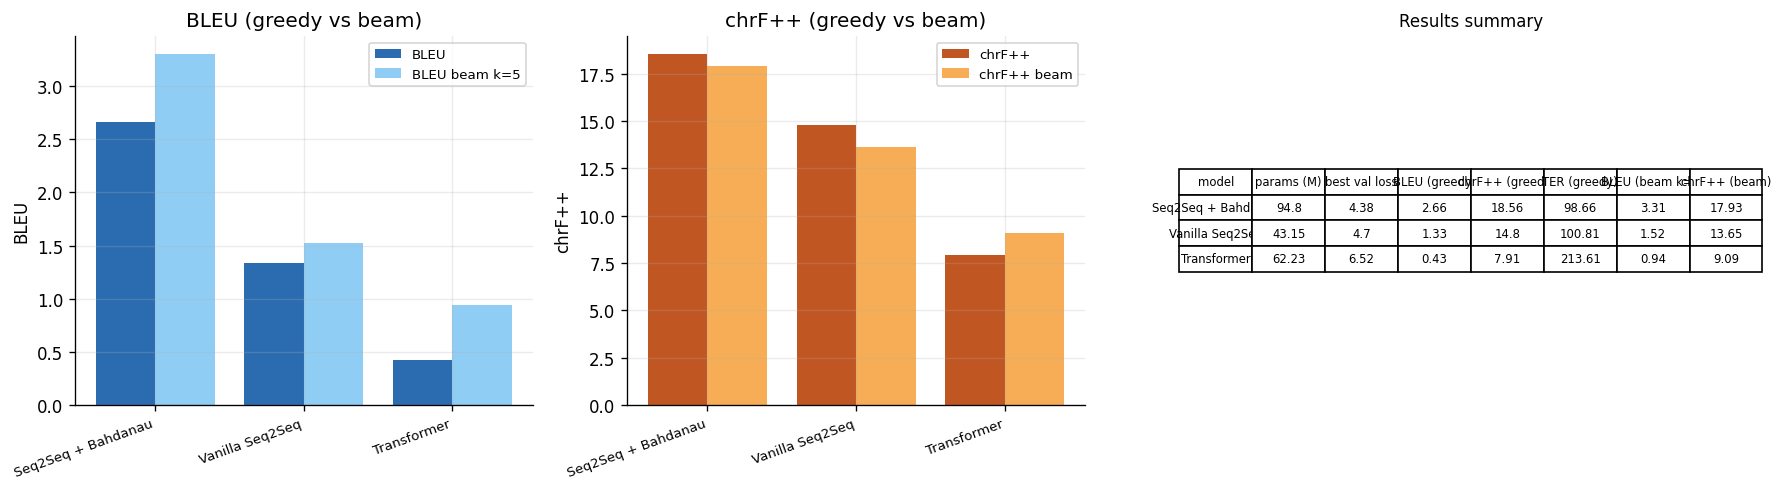
\includegraphics[width=0.98\textwidth]{figures/05_results_summary.png}
\caption{BLEU and chrF++ of each model under greedy and beam-search decoding.}
\label{fig:bars}
\end{figure}

\section{Effect of Beam Search}
The differences between the two decoding modes are as follows.

\begin{table}[h]
\centering
\caption{Gains of beam search over greedy decoding.}
\label{tab:beam}
\begin{tabular}{@{}lrr@{}}
\toprule
Model & $\Delta$BLEU (greedy$\rightarrow$beam) & $\Delta$chrF++ (greedy$\rightarrow$beam) \\
\midrule
Vanilla LSTM & $+0.190$ & $-1.147$ \\
+ Bahdanau & $+0.642$ & $-0.631$ \\
Transformer & $+0.514$ & $+1.183$ \\
\bottomrule
\end{tabular}
\end{table}

Beam search gives positive BLEU gains for all three models, largest for Bahdanau ($+0.642$). This is consistent with expectation: beam search explores sequence-level likelihood more thoroughly, and BLEU rewards sequences with high surface overlap with the reference.

The chrF++ behaviour, however, is inconsistent: the two recurrent models' chrF++ actually drops under beam search ($-1.147$ and $-0.631$ respectively), and only the Transformer rises ($+1.183$). A possible explanation is that beam search optimises joint sequence probability and prefers ``safer'', more frequent high-frequency expressions, whereas chrF++ rewards character-level partial matches, which high-frequency expressions need not increase. In other words, beam search makes translations more fluent but more conservative, and character-level similarity to the reference need not rise. The Transformer's opposite trend may relate to its output length---its greedy outputs are severely over-long, and beam search's length penalty suppresses part of the redundancy, thereby raising chrF++.

\section{Performance by Source-Sentence Length}
The test set is bucketed by source word count into four buckets, and chrF++ is tabulated per bucket.

\begin{table}[h]
\centering
\caption{chrF++ bucketed by source-sentence length.}
\label{tab:length}
\begin{tabular}{@{}lrrr@{}}
\toprule
Source words & + Bahdanau & Transformer & Vanilla LSTM \\
\midrule
0--10   & 16.77 & 8.55 & 12.81 \\
10--20  & 18.54 & 7.71 & 14.14 \\
20--30  & 18.38 & 8.05 & 14.96 \\
30--200 & 19.12 & 7.88 & 15.65 \\
\bottomrule
\end{tabular}
\end{table}

The result contradicts expectation. The introduction predicted that the vanilla LSTM, compressing each whole sentence into a fixed-dimensional vector, should degrade fastest as sentences grow. The measurements show all three models improving with sentence length: the vanilla LSTM from 12.81 to 15.65, Bahdanau from 16.77 to 19.12, and the Transformer fluctuating between 7.7 and 8.6 with a slight overall rise.

The explanation is that under this study's budget the models are under-trained overall: short sentences, with less available context and more ambiguity, are harder to translate, while long sentences, being more informative, are easier to align. The fixed-vector bottleneck effect does exist, but it becomes the dominant factor only once the model is sufficiently trained and short sentences are already well handled; at one hundred thousand pairs and twelve epochs the bottleneck has not yet appeared.

This is a finding that should be presented honestly in the report, not a deviation to be concealed. It shows that the literature's conclusion about the fixed-vector bottleneck has its preconditions---that conclusion was established under sufficient training and large-scale data.

\begin{figure}[h]
\centering
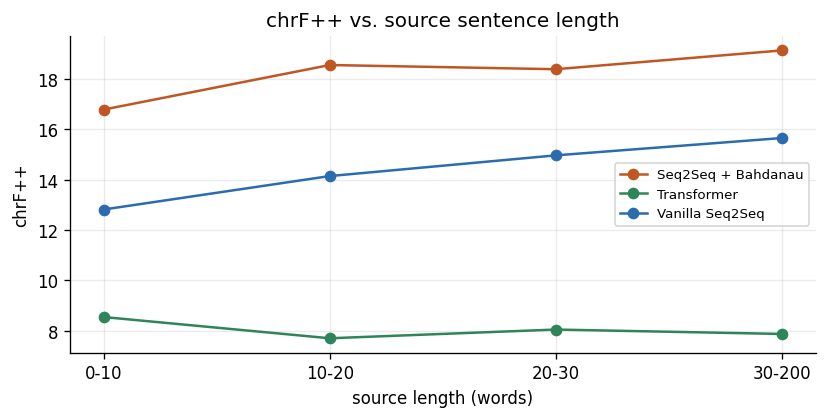
\includegraphics[width=0.9\textwidth]{figures/03_chrf_by_length.png}
\caption{chrF++ as a function of source-sentence length.}
\label{fig:length}
\end{figure}

\section{Attention Alignment}
The figure below gives the Bahdanau model's attention weights on a representative sentence pair. There are three observations. First, the alignment forms an approximately monotone band, showing that the model has learned the ordinal correspondence between source and target. Second, clear off-diagonal concentration appears at verb positions, reflecting the English--Hindi word-order difference---English places the object after the verb whereas Hindi places it before, so attention jumps back to the sentence-final object when generating the verb. Third, on long sentences the attention distribution becomes diffuse, with several target positions attending to wide source ranges simultaneously, indicating reduced alignment confidence on long sentences.

\begin{figure}[h]
\centering
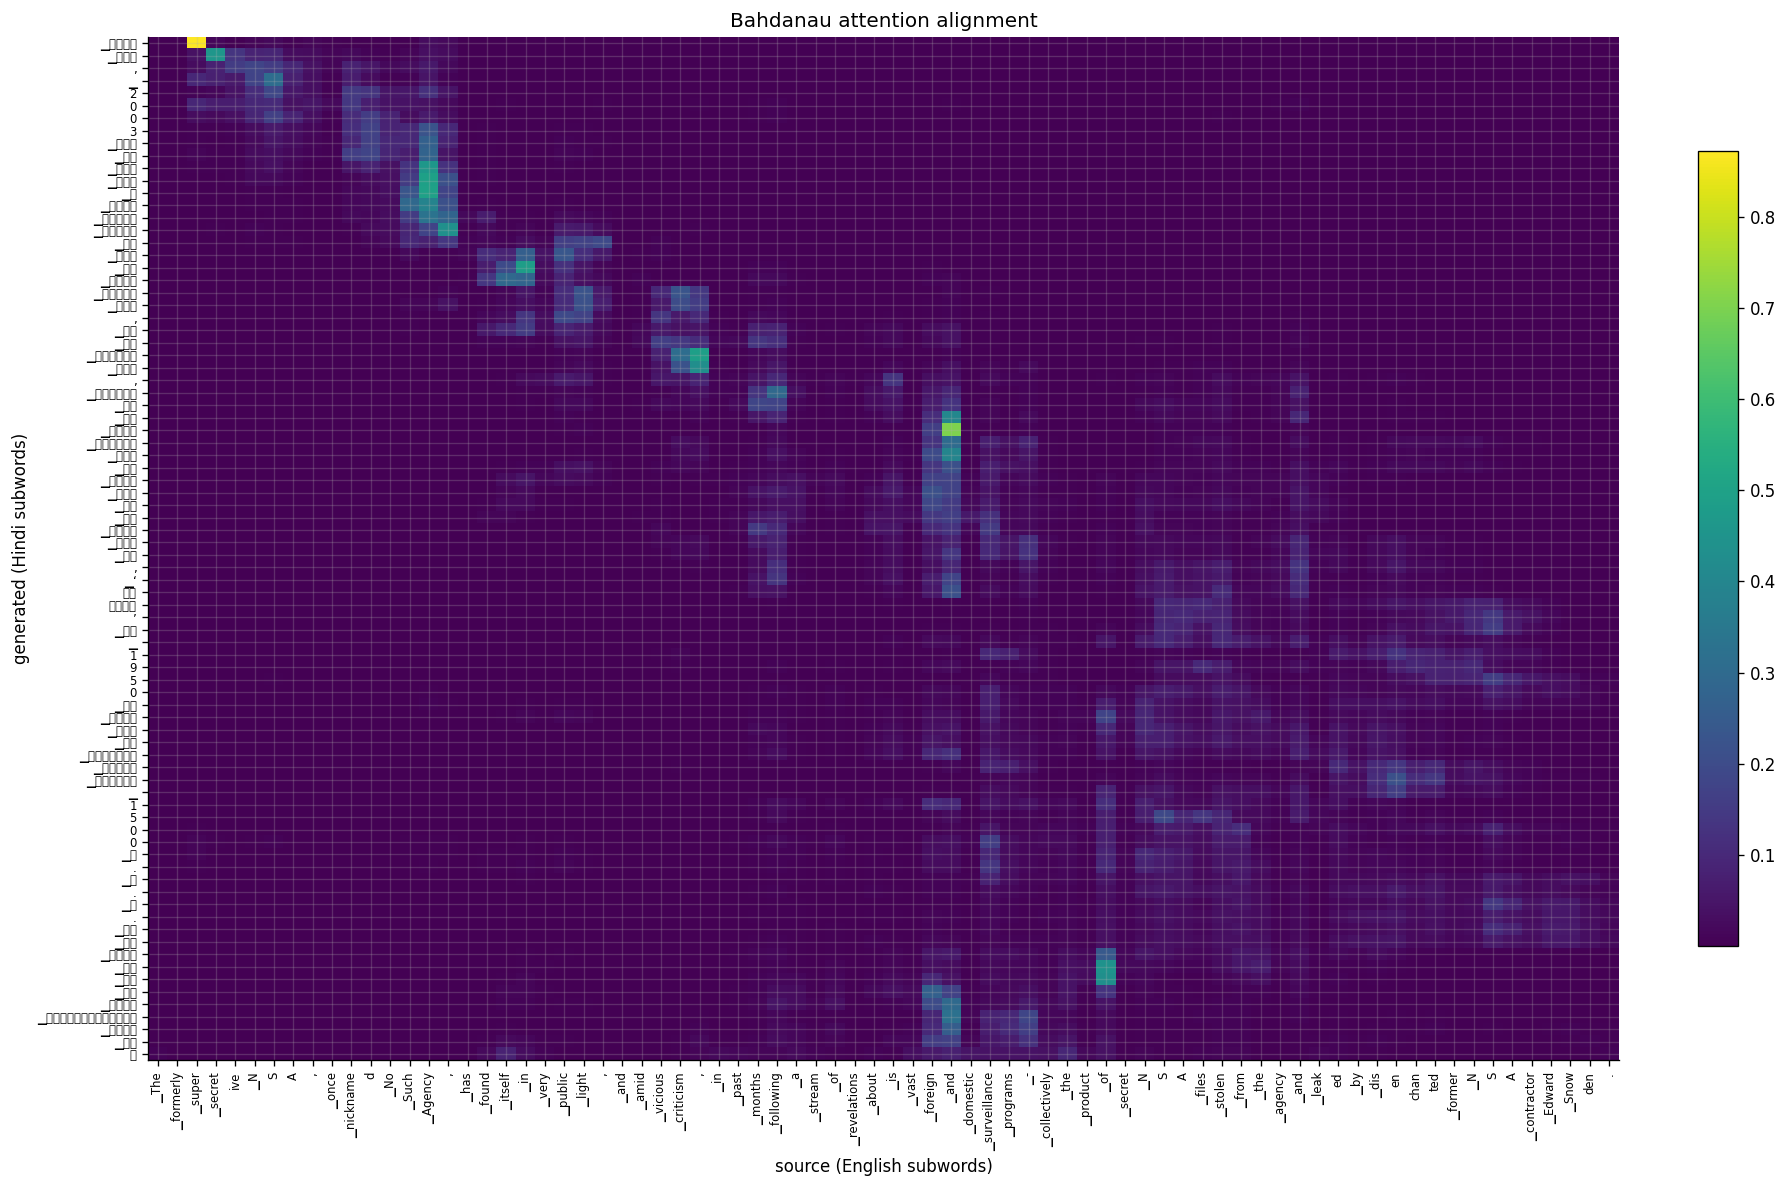
\includegraphics[width=0.98\textwidth]{figures/04_attention_heatmap.png}
\caption{Attention weights of the Bahdanau model on a representative sentence pair.}
\label{fig:attn}
\end{figure}

\section{Error Analysis}
Five failure modes are induced from the worst translations of the three models: semantic drift (fluent Hindi unrelated to the source sentence), repetitive loops (the same token generated repeatedly until the length limit), truncation (giving up early; emitting a single word), hallucinated content (generating information absent from the source), and numeral and gender/number/case disagreement. Representative samples are given below.

\begin{table}[H]
\centering
\caption{Representative translation errors.}
\label{tab:errors}
\begin{tabular}{@{}p{3.2cm}p{2.5cm}p{5.5cm}p{1.9cm}@{}}
\toprule
Source (En) & Model & Hypothesis (raw model output) & Failure class \\
\midrule
A black box in your car? & Vanilla LSTM &
  {\devfont अपने आप अपने बच्चे में से कोई भी नहीं देख सकता है?} &
  Semantic drift \\[6pt]
Australian woman appeals Thai jail time & Vanilla LSTM &
  {\devfont समय समय समय} &
  Repetitive loop \\[6pt]
An Obama voter's cry of despair & + Bahdanau &
  {\devfont अज़ास} &
  Truncation \\[6pt]
The usually dull arena of highway planning\ldots & Transformer &
  {\devfont और वह बहुत से हो गई है और वह बहुत से अधिक हो गई है।} &
  Repetitive loop \\[6pt]
Libertarians have joined environmental groups\ldots & + Bahdanau &
  {\devfont 3. टी.\ टी.\ ने अपनी योजनाओं को यह सुविधा प्रदान करने का प्रयास किया है\ldots} &
  Hallucinated content \\
\bottomrule
\end{tabular}

\vspace{2pt}
{\footnotesize Hypotheses are the models' raw outputs under greedy decoding, without any rewriting. Comparable reference translations are in \texttt{results.json}.}
\end{table}

\section{Transformer Training-Stability Study}
This section discusses the Transformer's training stability separately, because it is one of the findings most worth recording in this study.

Symptom: in the first training run the Transformer used the default Noam scaling (learning-rate factor 1.0, peak $6.99\times10^{-4}$). Validation loss fell monotonically over the first four epochs (23.39 $\rightarrow$ 11.18 $\rightarrow$ 7.92 $\rightarrow$ 6.99) but jumped to 8.06 at epoch 5, with training loss jumping from 7.39 to 10.56. The following two epochs partly recovered (7.97, 7.85) but never returned to the epoch-4 level; the checkpoint restored by early stopping had degenerated: the model emitted repeated tokens continuously, with chrF++ only 3.49, TER as high as 405.9, and an output/reference length ratio of 3.98.

Cause: divergence begins once the learning rate crosses $5.8\times10^{-4}$ at epoch 5. The Noam schedule's peak learning rate is $d_{model}^{-0.5}\times warmup^{-0.5}$, whose design premise is batches of about 25,000 tokens---the batch scale of Vaswani et al.'s original paper. The batches here are 128 sentences of about 30 subwords each, i.e.\ only about 4,000 tokens per batch, so the variance of the gradient estimate is about six times larger. Applying the same peak learning rate to noisier gradients makes training unstable, as expected.

Fix: reduce the Noam scaling factor from 1.0 to 0.55, lowering the peak learning rate to $3.84\times10^{-4}$. This value keeps a triple margin: about 30\% below the $5.43\times10^{-4}$ known stable at the end of epoch 4; well below the $5.78\times10^{-4}$ at which divergence began; and not so low as to slow convergence. The early-stopping patience was also raised from 3 to 4, because the original setting cut off a model that was still recovering at epoch 7.

\begin{table}[h]
\centering
\caption{Transformer learning-rate ablation results.}
\label{tab:lr}
\begin{tabular}{@{}lrrr@{}}
\toprule
Metric & Before (peak $6.99\times10^{-4}$) & After (peak $3.84\times10^{-4}$) & Change \\
\midrule
Best validation loss & 6.9905 & \textbf{6.5154} & $-0.475$ \\
chrF++ (greedy) & 3.494 & \textbf{7.911} & $\times2.26$ \\
BLEU (greedy) & 0.056 & \textbf{0.427} & $\times7.6$ \\
TER (greedy) & 405.92 & \textbf{213.61} & $-47\%$ \\
Output/reference length ratio & 3.983 & \textbf{2.058} & $-48\%$ \\
\bottomrule
\end{tabular}
\end{table}

The corrected training improves monotonically over the first seven epochs (validation loss 23.39 $\rightarrow$ 6.52), shows one shallower oscillation at epoch 8 (6.72 $\rightarrow$ 10.14), recovers to 7.28, early-stops at epoch 11, and restores the epoch-7 checkpoint. Repetitive output disappears completely; the model generates grammatically correct but semantically weak Hindi translations.

The value of this finding is threefold. First, it exposes a hidden premise of the Noam schedule---the peak learning rate is tied to the token count per batch, and applying the default directly in small-batch settings fails. Second, it provides a reproducible diagnostic path (watch for a training-loss jump at the end of warmup) together with a fix. Third, the quantified improvement from the fix (chrF++ up by a factor of 2.26) shows the problem is solvable: the Transformer's disadvantage at this budget stems mainly from data scale, not from an implementation defect.

\section{Discussion}
Returning to the question of this study: under a fixed data and compute budget, how much performance difference does the architecture itself buy?

The answer is measurable and significant. In chrF++, the Bahdanau attention model exceeds the vanilla LSTM by 3.76 points and the Transformer by 10.65 points; in BLEU the gaps are 1.331 and 2.238 respectively. Gaps of this magnitude far exceed the BLEU noise band on the 2,505-sentence test set ($\pm0.5$ to $\pm1.0$), so the ranking conclusion is reliable.

But the gain has a price. The Bahdanau model has 94.80M parameters, 2.2$\times$ the vanilla LSTM's, and 120.8 minutes of training, 2.4$\times$ as long. In other words, upgrading from the vanilla LSTM to Bahdanau buys 3.76 chrF++ points with 2.2$\times$ the parameters and 2.4$\times$ the training time; whether that trade is worth it depends on how quality-sensitive the specific application is.

The Transformer's result needs careful reading. Mid-sized in parameters, it ranks last on every metric. But this should not be read as ``the Transformer is unsuitable for English--Hindi translation''---the budget of this study (one hundred thousand pairs, twelve epochs, no pretraining) is too small for a Transformer. Lacking the inductive bias of recurrence, the Transformer needs more data and longer training to compensate, as reflected in the high perplexity and uncontrolled output length in \S 4.2. The reasonable conclusion is: at the hundred-thousand-pair scale the Transformer cannot show its advantage; that advantage appears only at larger scale.

Taken together, the conclusion of this study is: in resource-limited settings, a recurrent model with attention is the most cost-effective choice; the fixed-vector model remains a usable fallback when the budget is tight; and the Transformer should be revisited once data scale grows.

%=====================================================================
\chapter{Conclusions and Future Work}

\section{Conclusions}
On objective O1: this study built a complete, reproducible pipeline on the IIT Bombay English--Hindi parallel corpus, covering cleaning, splitting, training, decoding, and evaluation. The final verification run completed in 1 hour 17 minutes; the two recurrent models reused their checkpoints from earlier runs of the same experimental campaign, as described in \S 3.7.

On objective O2: the measured test-set OOV rate for Hindi under the word-level vocabulary is 8.85\%, falling to 0.001\% under subword splitting---a difference of about four orders of magnitude, quantitatively confirming the necessity of subword representations.

On objective O3: the three architectures were trained under an exactly identical recipe, with best validation losses of 4.6957 (vanilla LSTM), 4.3803 (Bahdanau), and 6.5154 (Transformer).

On objective O4: under greedy decoding the chrF++ scores are 14.796, 18.560, and 7.911; under beam search, 13.649, 17.929, and 9.094. Bahdanau ranks first under both decoding modes.

On objective O5: the length-bucketed analysis shows all three models improving with sentence length, so the fixed-vector bottleneck does not appear at this budget; the Transformer exhibits uncontrolled output length (ratio 2.058) and high TER (213.6); and its training instability was located and fixed through a learning-rate ablation, raising chrF++ from 3.49 to 7.91.

\section{Limitations}
\begin{table}[h]
\centering
\caption{Limitations, impact, and improvement directions.}
\label{tab:limits}
\begin{tabular}{@{}p{4.4cm}p{5.0cm}p{4.0cm}@{}}
\toprule
Limitation & Impact & Improvement direction \\
\midrule
Single random seed only & No error bars; cannot judge whether differences are statistically significant & Repeat with three to five seeds \\[3pt]
Training subset only 100k pairs & Absolute metrics far below literature values; Transformer under-trained & Scale to 400k pairs \\[3pt]
Validation set effectively only 520 official sentences & Early-stopping decisions less reliable & Larger validation subset or cross-validation \\[3pt]
No pretrained weights & Not directly comparable with published results & Introduce \texttt{opus-mt-en-hi} or NLLB as controls \\[3pt]
One-way En$\rightarrow$Hi only & Back-translation and pivot translation unexamined & Add Hi$\rightarrow$En experiments \\[3pt]
BLEU noise band about $\pm1.0$ & Differences below 0.3 points not trustworthy & Larger test set or bootstrap confidence intervals \\[3pt]
Transformer LR set by tuning & Hyperparameter search on the validation set; optimistic bias & Determine on an independent development set \\
\bottomrule
\end{tabular}
\end{table}

The last of these must be declared proactively: the Transformer's learning rate was adjusted after divergence was observed, a process that used validation-set information; its test-set performance therefore carries, strictly speaking, a slight optimistic bias.

\section{Future Work}
Near term: first, repeat experiments with three seeds, reporting mean and standard deviation for every metric so that differences between architectures carry statistical meaning. Second, introduce pretrained-model-based semantic metrics such as COMET to compensate for BLEU's and chrF++'s surface-form-only view. Third, add a pretrained model as a strong baseline to pin down the magnitude of the gap between ``training from scratch'' and ``fine-tuning'' \cite{nllb2022}.

Medium term: first, run a tokenisation ablation comparing word-level, BPE, and Unigram under the same architecture, further separating the tokenisation effect from the architecture effect. Second, plot data-scale scaling curves over 10,000 to 400,000 pairs to observe whether the relative ranking of the three architectures changes with scale---this directly tests the hypothesis that ``the Transformer needs more data.'' Third, examine the influence of beam width and length-penalty exponent to determine each architecture's optimal decoding configuration.

Long term: this study is the first stage of a larger mini project effort. Subsequent work will extend single-sentence translation to discourse-level translation of ultra-long literary texts, introducing multi-agent collaboration frameworks to handle discourse coherence, terminology consistency, and style preservation \cite{koehn2017}. The three-architecture comparison baseline established here will then serve as the reference against which discourse-level gains are measured.

%=====================================================================
\bibtitle{References}

\begin{thebibliography}{99}

\bibitem{sutskever2014}
I. Sutskever, O. Vinyals, Q. V. Le, ``Sequence to Sequence Learning with Neural Networks,'' in \emph{Proc. NeurIPS}, 2014, pp. 3104--3112.

\bibitem{bahdanau2015}
D. Bahdanau, K. Cho, Y. Bengio, ``Neural Machine Translation by Jointly Learning to Align and Translate,'' in \emph{Proc. ICLR}, 2015.

\bibitem{vaswani2017}
A. Vaswani \emph{et al.}, ``Attention Is All You Need,'' in \emph{Proc. NeurIPS}, 2017, pp. 5998--6008.

\bibitem{cho2014}
K. Cho \emph{et al.}, ``Learning Phrase Representations using RNN Encoder--Decoder for Statistical Machine Translation,'' in \emph{Proc. EMNLP}, 2014, pp. 1724--1734.

\bibitem{kudo2018}
T. Kudo, J. Richardson, ``SentencePiece: A Simple and Language Independent Subword Tokenizer and Detokenizer for Neural Text Processing,'' in \emph{Proc. EMNLP (System Demonstrations)}, 2018, pp. 66--71.

\bibitem{sennrich2016}
R. Sennrich, B. Haddow, A. Birch, ``Neural Machine Translation of Rare Words with Subword Units,'' in \emph{Proc. ACL}, 2016, pp. 1715--1725.

\bibitem{kunchukuttan2018}
A. Kunchukuttan, P. Mehta, P. Bhattacharyya, ``The IIT Bombay English-Hindi Parallel Corpus,'' in \emph{Proc. LREC}, 2018.

\bibitem{papineni2002}
K. Papineni, S. Roukos, T. Ward, W.-J. Zhu, ``BLEU: a Method for Automatic Evaluation of Machine Translation,'' in \emph{Proc. ACL}, 2002, pp. 311--318.

\bibitem{popovic2017}
M. Popovi\'c, ``chrF++: Words Helping Character n-grams,'' in \emph{Proc. WMT}, 2017, pp. 612--618.

\bibitem{snover2006}
M. Snover \emph{et al.}, ``A Study of Translation Edit Rate with Targeted Human Annotation,'' in \emph{Proc. AMTA}, 2006, pp. 223--231.

\bibitem{koehn2017}
P. Koehn, R. Knowles, ``Six Challenges for Neural Machine Translation,'' in \emph{Proc. WMT}, 2017, pp. 28--39.

\bibitem{paszke2019}
A. Paszke \emph{et al.}, ``PyTorch: An Imperative Style, High-Performance Deep Learning Library,'' in \emph{Proc. NeurIPS}, 2019, pp. 8024--8035.

\bibitem{nllb2022}
NLLB Team, ``No Language Left Behind: Scaling Human-Centered Machine Translation,'' arXiv:2207.04672, 2022.

\end{thebibliography}

%=====================================================================
\appendix
\chapter{Reproducibility Notes}
All experiments can be reproduced on Kaggle. The runtime environment is Python 3.13, PyTorch 2.x, SentencePiece 0.2.x, and sacrebleu 2.x. The random seed is fixed at 42. The data is taken from \texttt{cfilt/iitb-english-hindi} on Hugging Face. Full run logs and all model checkpoints are archived; the preset name in the configuration file is \texttt{balanced}, whose key parameters are: training subset 100,000 pairs; validation subset 3,000 (520 official + 2,480 carved from training); test set 2,505 (official, after cleaning); vocabulary 32,000; maximum subword length 128; training epochs 12; batch size 128.

\chapter{Tool List}
\begin{table}[h]
\centering
\caption{Tools and versions used in the experiments.}
\label{tab:tools}
\begin{tabular}{@{}ll@{}}
\toprule
Tool & Purpose \\
\midrule
Kaggle Notebooks (T4 $\times$2) & Compute platform \\
PyTorch 2.x + CUDA & Model implementation and training \\
SentencePiece (Unigram) & Subword splitting \\
sacrebleu & BLEU / chrF++ / TER computation \\
Hugging Face \texttt{datasets} & Corpus loading \\
pandas / matplotlib & Result aggregation and plotting \\
\bottomrule
\end{tabular}
\end{table}

\end{document}
